\chapter{Reaction Rates}\label{ch:g12:reaction-rates}

A bottle of milk left on the kitchen counter turns sour in a couple of
days; in the fridge, it keeps for more than a week. A firework burns in a
fraction of a second, while a limestone statue in a city park weathers
over centuries. \omterm{def:g8:balanced-equations:equation}{Balanced equations} and \omterm{def:g10:reaction-progress-table:extent}{progress tables} say what a
reaction gives and how much; they say nothing about how fast. This
chapter measures the speed of reactions, finds what controls it, and
describes the simplest way a reaction can slow down as it goes.

\begin{recall}
The concentration of a solution (\cref{ch:g10:concentration-and-dilution})
and the extent of a reaction (\cref{ch:g10:reaction-progress-table}). The
\omterm{def:g11:absorbance:absorbance}{absorbance} of a dilute solution is proportional to the concentration of
the coloured species (\cref{ch:g11:absorbance}). A \omterm{def:g11:titration:titration}{titration} measures the
amount of a species (\cref{ch:g11:titration}).
\end{recall}

\begin{omfigure}
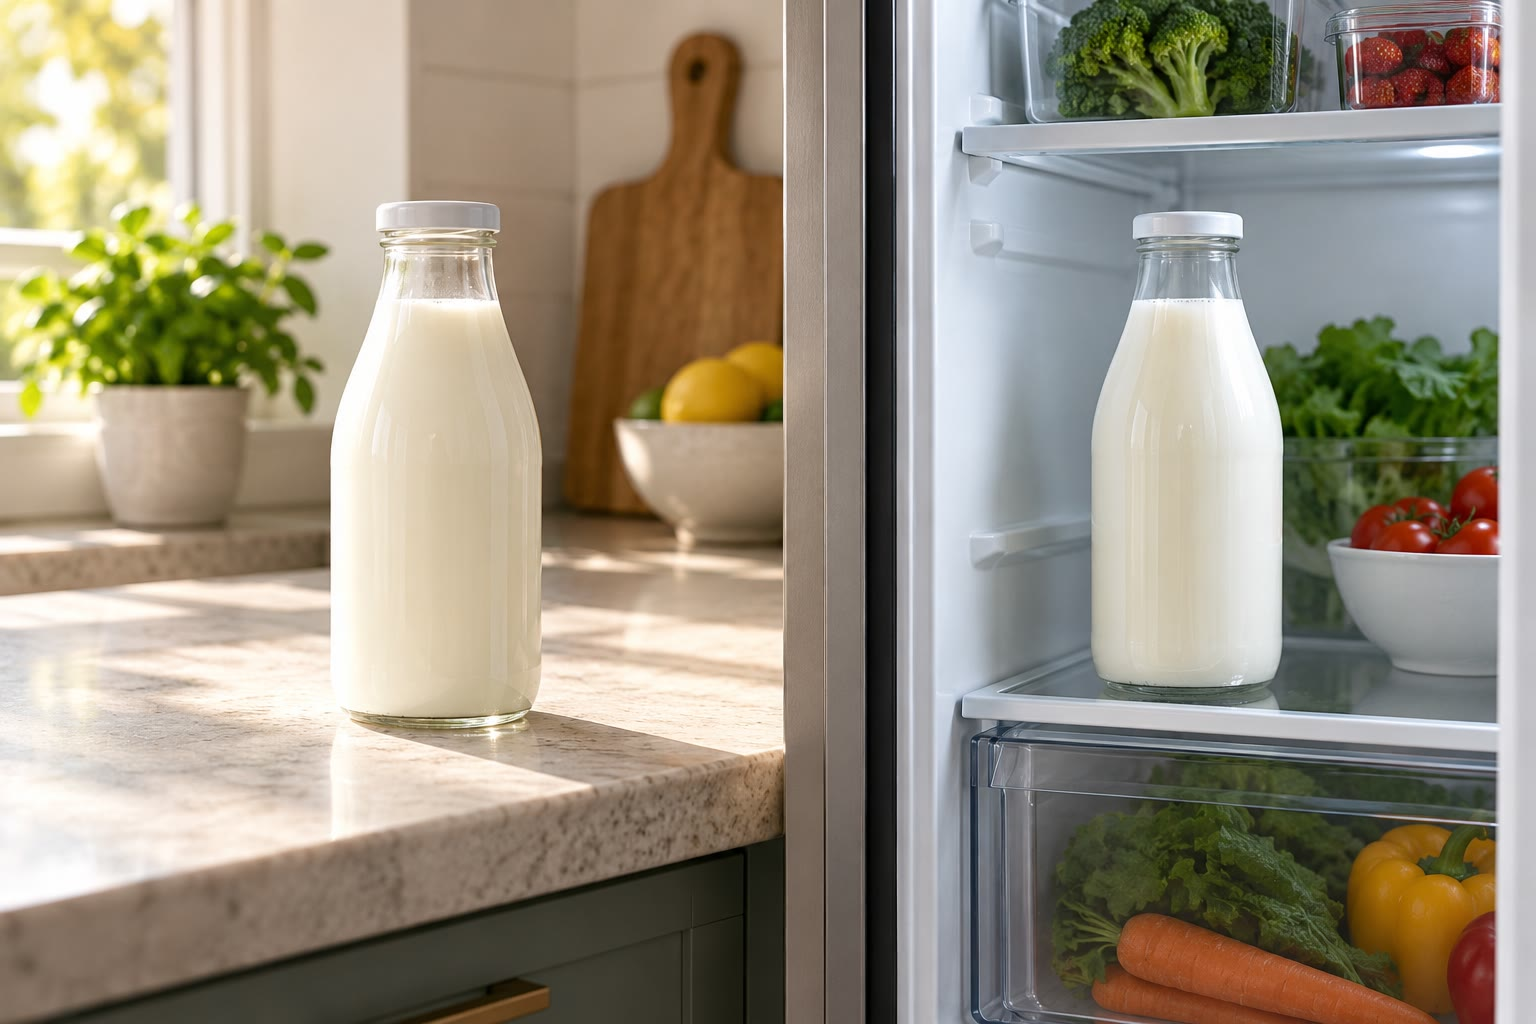
\includegraphics[width=0.48\linewidth]{images/book1/ai/g12-milk-counter-fridge.jpg}

{\small The same milk, on the counter and in the fridge: the reactions
that sour it are slower in the cold.}
\end{omfigure}

\section{Following a reaction in time}

Some reactions are over as soon as the \omterm{def:g7:chemical-reactions:reactant}{reactants} meet: the \omterm{def:g9:ions:precipitate}{precipitation}
of silver chloride, the reaction of an acid with a base. Others take
minutes, hours or years. To study a slow reaction, chemists measure the
concentration of a \omterm{def:g7:chemical-reactions:reactant}{reactant} or a product at regular times. They can
\begin{itemize}
  \item take small samples, stop the reaction in each, and titrate them;
  \item measure the \omterm{def:g11:absorbance:absorbance}{absorbance} of the solution, when a \omterm{def:g7:chemical-reactions:reactant}{reactant} or a
        product is coloured;
  \item measure the pressure or the volume of a gas given off, or the
        conductivity of a solution whose \omterm{def:g9:ions:ion}{ions} change.
\end{itemize}

\begin{definition}[Quenching]\label{def:g12:reaction-rates:quenching}
\emph{Quenching}\index{quenching} a sample is stopping, or very greatly
slowing, the reaction in it at the moment it is taken, usually by
cooling it suddenly and diluting it, so that its composition can be
measured at leisure.
\end{definition}

\begin{inthelab}[Quenching a sample]
Every five minutes, \qty{10.0}{mL} of the reaction \omterm{def:g6:pure-substances-and-mixtures:mixture}{mixture} are taken with
a pipette and poured into a beaker holding about \qty{50}{mL} of
ice-cold water. Diluted five times and cooled close to
\qty{0}{\celsius}, the reaction becomes so slow that it can be considered
stopped; the sample is then titrated. The time of the sample is the time
it was poured into the ice water, not the time of the \omterm{def:g11:titration:titration}{titration}.
\end{inthelab}

\begin{omfigure}
\begin{tikzpicture}[font=\small, scale=0.8]
  \pic[transform shape] at (0,0) {erlenmeyer={0.4}{orange!25}};
  \node[anchor=north, align=center] at (0,-0.15) {reaction\\ mixture};
  \pic[transform shape, rotate=-35] at (1.4,1.2) {pipette={0.6}{orange!25}};
  \draw[omProp, very thick, -{Stealth}] (1.6,0.8) -- (2.9,0.8);
  \node[anchor=south] at (2.25,0.85) {\qty{10.0}{mL}};
  \pic[transform shape] at (4,0) {beaker={0.55}{cyan!12}};
  \foreach \p in {(3.6,0.4),(4.2,0.6),(3.9,0.85),(4.4,0.3)}
    \draw[black!30, fill=white] \p ++(-0.1,-0.08) rectangle ++(0.2,0.16);
  \node[anchor=north, align=center] at (4,-0.15) {ice-cold water:\\ reaction stopped};
  \draw[omProp, very thick, -{Stealth}] (5.1,0.8) -- (6.4,0.8);
  \pic[transform shape] at (7.5,0) {erlenmeyer={0.35}{orange!12}};
  \pic[transform shape] at (7.5,2.75) {burette={0.7}{violet!45}};
  \node[anchor=north, align=center] at (7.5,-0.15) {titration of\\ the sample};
\end{tikzpicture}

{\small Following a reaction by sampling: take a sample, quench it, then
measure it at leisure.}
\end{omfigure}

\section{Kinetic factors}

\begin{definition}[Kinetic factor]\label{def:g12:reaction-rates:kinetic-factor}
A \emph{kinetic factor}\index{kinetic factor} is a quantity that changes
the speed of a reaction without changing what the reaction gives: the
temperature, the concentrations of the \omterm{def:g7:chemical-reactions:reactant}{reactants}, the area of contact
between \omterm{def:g7:chemical-reactions:reactant}{reactants} in different phases, and the presence of a catalyst
(next chapter).
\end{definition}

\begin{proposition}[Hotter, more concentrated, finer: faster]\label{prop:g12:reaction-rates:factors}
In general a reaction is faster when the temperature is higher, when the
\omterm{def:g7:chemical-reactions:reactant}{reactants} are more concentrated, and, for a solid \omterm{def:g7:chemical-reactions:reactant}{reactant}, when it is
more finely divided.
\end{proposition}

\begin{proof}
Admitted, with a picture: reacting particles must meet, and meet hard
enough. Concentrating them makes meetings more frequent; dividing a solid
offers more surface to meet; heating makes them move faster, so that they
meet more often and, above all, more of the meetings are energetic enough
to break bonds.
\end{proof}

\begin{example}[Three everyday cases]\label{ex:g12:reaction-rates:everyday}
Food keeps longer in the fridge and much longer in the freezer: the
reactions that spoil it slow down in the cold. Fine flour dust in the \omterm{def:g4:air-a-mixture-of-gases:air}{air}
of a mill can explode, while a sack of flour only smoulders: same
reaction, enormous contact area. A tablet that fizzes in water \omterm{def:g2:mixing-and-dissolving:dissolve}{dissolves}
faster if it is crushed first.
\end{example}

\begin{omfigure}
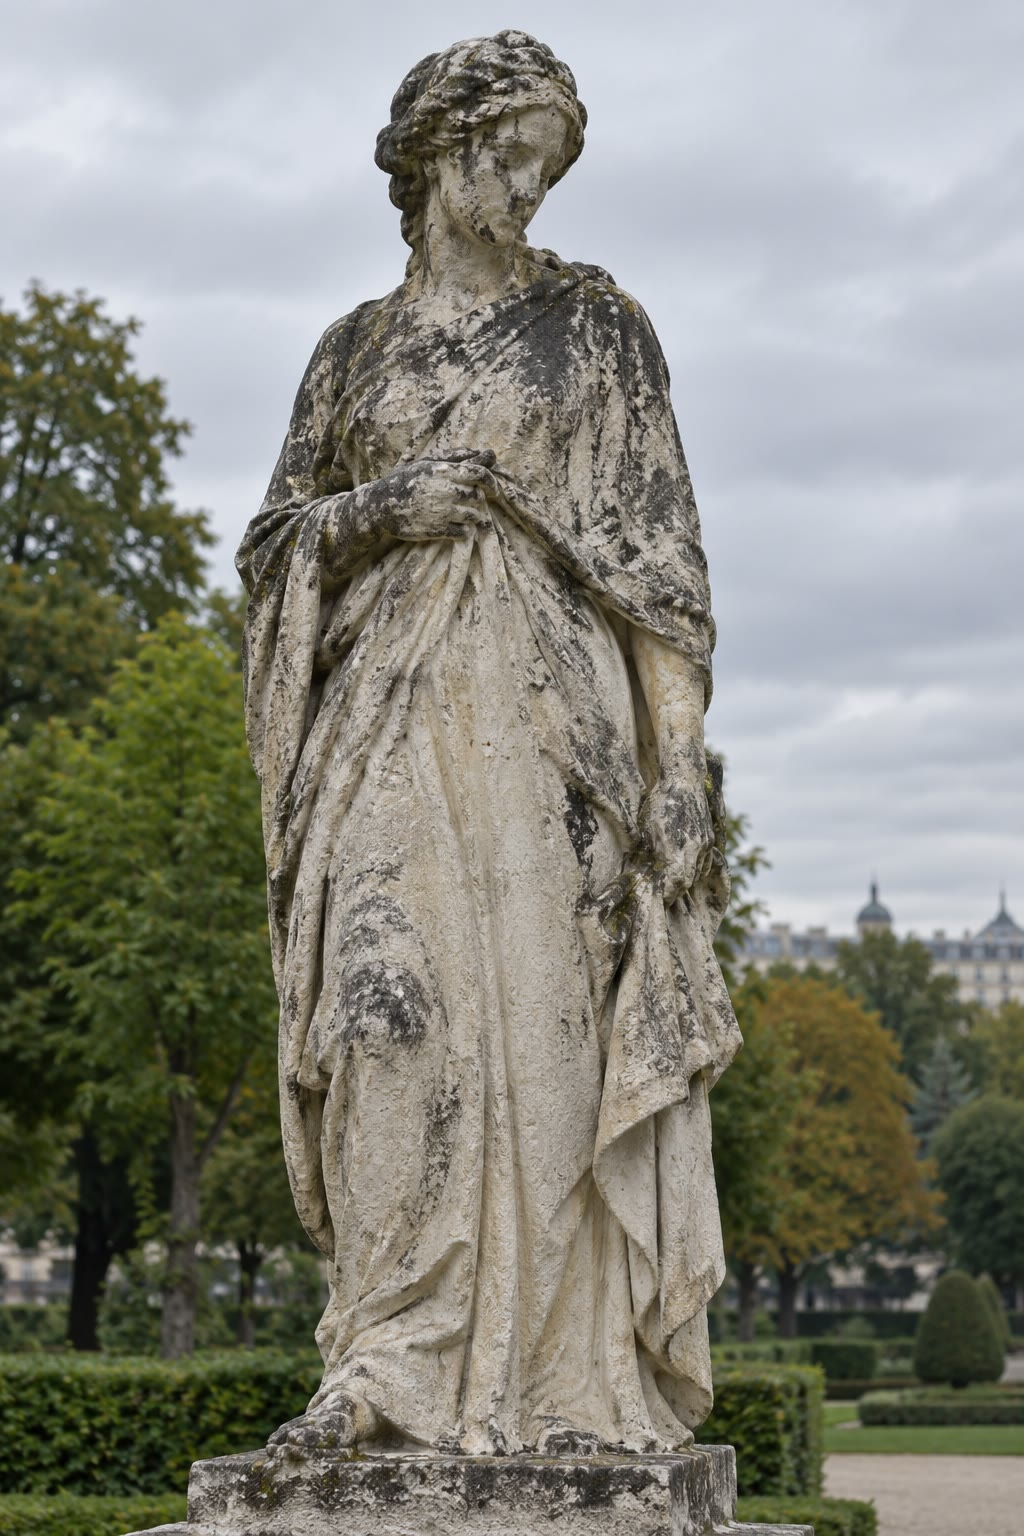
\includegraphics[width=0.42\linewidth,height=6cm,keepaspectratio]{images/book1/ai/g12-weathered-statue.jpg}

{\small A limestone statue weathered by rain: a reaction that takes
centuries.}
\end{omfigure}

\section{Rates of disappearance and of appearance}

\begin{definition}[Rate of disappearance, rate of appearance]\label{def:g12:reaction-rates:rate}
In a solution of constant volume, the \emph{rate of disappearance}\index{rate
of disappearance} of a \omterm{def:g7:chemical-reactions:reactant}{reactant} A at time $t$ is
\[
  v_A(t) = -\frac{d[\ce{A}]}{dt},
\]
and the \emph{rate of appearance}\index{rate of appearance} of a product
P is $v_P(t) = \dfrac{d[\ce{P}]}{dt}$. Both are positive, in
\si{mol.L^{-1}.min^{-1}} (or per second).
\end{definition}


\begin{method}[Reading a rate from a tangent]\label{met:g12:reaction-rates:tangent}
\begin{enumerate}
  \item On the curve of $[\ce{A}]$ against $t$, draw the tangent at the
        chosen time.
  \item Read two points far apart on the tangent and compute its slope,
        $\Delta[\ce{A}] / \Delta t$.
  \item The \omterm{def:g12:reaction-rates:rate}{rate of disappearance} is the opposite of this slope (for a
        product, the slope itself).
\end{enumerate}
\end{method}

\begin{omfigure}
\begin{tikzpicture}
\begin{axis}[width=0.8\linewidth, height=6.4cm, xmin=0, xmax=60, ymin=0,
    ymax=11, xlabel={$t$ (\si{min})}, ylabel={$[\ce{A}]$ (\si{mmol/L})},
    axis lines*=left, ymajorgrids, xmajorgrids, grid style={gray!20},
    tick label style={font=\small}, label style={font=\small},
    legend style={font=\small, at={(0.98,0.97)}, anchor=north east,
    draw=none, fill=white}, legend cell align=left]
  \addplot[very thick, omDef] table[x=t, y=A1] {figdata/out/grade-12-reaction-rates-a.dat};
  \addplot[very thick, omThm] table[x=t, y=A2] {figdata/out/grade-12-reaction-rates-a.dat};
  \addplot[thick, dashed, omProp, restrict y to domain=0:11] table[x=t, y=tangent]
    {figdata/out/grade-12-reaction-rates-a.dat};
  \legend{$k = \qty{0.050}{min^{-1}}$, $k = \qty{0.100}{min^{-1}}$ (warmer),
    tangent at $t = 0$}
  \addplot[densely dotted, black!60] coordinates {(0,5) (13.86,5) (13.86,0)};
  \addplot[densely dotted, black!60] coordinates {(6.93,5) (6.93,0)};
  \node[font=\small, anchor=south west] at (axis cs:14.6,5.4) {$t_{1/2} = \qty{13.9}{min}$};
  \node[font=\small, anchor=south east] at (axis cs:6.7,0.2) {\qty{6.9}{min}};
\end{axis}
\end{tikzpicture}

{\small The concentration of a \omterm{def:g7:chemical-reactions:reactant}{reactant} A against time, for the same
\omterm{def:g12:reaction-rates:first-order}{first-order reaction} at two temperatures. The tangent at $t = 0$ (dashed)
gives the initial rate; the dotted lines mark the half-lives.}
\end{omfigure}

\begin{example}[The initial rate]\label{ex:g12:reaction-rates:initial}
On the blue curve, the tangent at $t = 0$ goes from \qty{10.0}{mmol/L} at
$t = 0$ to $0$ at $t = \qty{20}{min}$: its slope is
$-10.0/20 = \qty{-0.50}{mmol.L^{-1}.min^{-1}}$, so the initial \omterm{def:g12:reaction-rates:rate}{rate of
disappearance} is \qty{0.50}{mmol.L^{-1}.min^{-1}}. Later the curve flattens
and the rate falls: the reaction slows down as A is used up.
\end{example}

\section{First-order reactions}

\begin{definition}[First-order reaction, rate constant]\label{def:g12:reaction-rates:first-order}
A reaction is a \emph{first-order reaction}\index{first-order reaction}
with respect to A if its \omterm{def:g12:reaction-rates:rate}{rate of disappearance} is proportional to the
concentration of A at every moment:
\[
  -\frac{d[\ce{A}]}{dt} = k\,[\ce{A}] .
\]
The positive constant $k$, in \si{min^{-1}} or \si{s^{-1}}, is the
\emph{rate constant}\index{rate constant}; it depends on the temperature.
\end{definition}

\begin{proposition}[Exponential decay]\label{prop:g12:reaction-rates:exponential}
For a \omterm{def:g12:reaction-rates:first-order}{first-order reaction} with initial concentration $[\ce{A}]_0$,
\[
  [\ce{A}](t) = [\ce{A}]_0\, e^{-kt} .
\]
\end{proposition}

\begin{proof}
The function $f(t) = [\ce{A}]_0 e^{-kt}$ has derivative
$f'(t) = -k [\ce{A}]_0 e^{-kt} = -k f(t)$, so it satisfies the rate
equation, and $f(0) = [\ce{A}]_0$. That it is the only such function is
admitted here (it is proved in mathematics, for equations $y' = ay$).
\end{proof}

\begin{method}[Testing for first order]\label{met:g12:reaction-rates:test}
\begin{enumerate}
  \item From the measurements, compute $\ln [\ce{A}]$ (or $\ln A$ for an
        \omterm{def:g11:absorbance:absorbance}{absorbance} proportional to $[\ce{A}]$) at each time.
  \item Plot $\ln[\ce{A}]$ against $t$: since
        $\ln[\ce{A}] = \ln[\ce{A}]_0 - kt$, the points lie on a straight
        line if and only if the reaction is first order.
  \item The slope of the line is $-k$.
\end{enumerate}
\end{method}

\section{Half-life}

\begin{definition}[Half-life]\label{def:g12:reaction-rates:half-life}
The \emph{half-life}\index{half-life} $t_{1/2}$ of a reaction is the time
it takes for the concentration of the \omterm{def:g10:reaction-progress-table:limiting}{limiting reactant} to fall to half
of its initial value.
\end{definition}

\begin{proposition}[Half-life of a first-order reaction]\label{prop:g12:reaction-rates:half-life}
For a \omterm{def:g12:reaction-rates:first-order}{first-order reaction},
\[
  t_{1/2} = \frac{\ln 2}{k},
\]
whatever the initial concentration; after $n$ half-lives, the
concentration is divided by $2^n$.
\end{proposition}

\begin{proof}
$[\ce{A}]_0 e^{-k t_{1/2}} = [\ce{A}]_0 / 2$ gives $e^{-k t_{1/2}} = 1/2$,
so $k t_{1/2} = \ln 2$. Each further \omterm{def:g12:reaction-rates:half-life}{half-life} multiplies the
concentration by $e^{-k t_{1/2}} = 1/2$ again.
\end{proof}


\begin{example}[Reading the half-lives]\label{ex:g12:reaction-rates:half-lives}
For $k = \qty{0.050}{min^{-1}}$, $t_{1/2} = 0.693 / 0.050 =
\qty{13.9}{min}$: the concentration falls from 10.0 to 5.0, then 2.5,
then \qty{1.25}{mmol/L} at 13.9, 27.7 and \qty{41.6}{min}. The warmer run,
with $k$ twice as large, has half the \omterm{def:g12:reaction-rates:half-life}{half-life}, \qty{6.9}{min}, as the
figure shows.
\end{example}

\begin{remark}[Half-lives elsewhere]\label{rem:g12:reaction-rates:radioactive}
The same word is used in physics for radioactive nuclei, whose number
falls in the same exponential way: a radioactive decay behaves like a
\omterm{def:g12:reaction-rates:first-order}{first-order reaction}. The physics book treats it.
\end{remark}

\begin{omfigure}
\begin{minipage}{0.49\linewidth}
\begin{tikzpicture}
\begin{axis}[width=\linewidth, height=5.4cm, xmin=0, xmax=26, ymin=0,
    ymax=0.85, xlabel={$t$ (\si{min})}, ylabel={absorbance $A$},
    axis lines*=left, ymajorgrids, grid style={gray!20},
    tick label style={font=\scriptsize}, label style={font=\small}]
  \addplot[only marks, mark=*, mark size=1.8pt, omDef] table[x=t, y=A]
    {figdata/out/grade-12-reaction-rates-b.dat};
  \addplot[thick, omProp, domain=0:26, samples=60] {0.8*exp(-0.11552*x)};
\end{axis}
\end{tikzpicture}
\end{minipage}\hfill
\begin{minipage}{0.49\linewidth}
\begin{tikzpicture}
\begin{axis}[width=\linewidth, height=5.4cm, xmin=0, xmax=26, ymin=-3.4,
    ymax=0, xlabel={$t$ (\si{min})}, ylabel={$\ln A$}, axis lines*=left,
    ymajorgrids, grid style={gray!20}, tick label style={font=\scriptsize},
    label style={font=\small}]
  \addplot[only marks, mark=*, mark size=1.8pt, omDef] table[x=t, y=lnA]
    {figdata/out/grade-12-reaction-rates-b.dat};
  \addplot[thick, omProp, domain=0:26] {-0.2231-0.11552*x};
\end{axis}
\end{tikzpicture}
\end{minipage}

{\small The fading of crystal violet in a \omterm{def:g9:acids-bases-ph:acidic}{basic solution} (data of the
weekend problem). Left: the \omterm{def:g11:absorbance:absorbance}{absorbance} falls along an exponential.
Right: $\ln A$ against $t$ is a straight line of slope
$-\qty{0.116}{min^{-1}}$: the reaction is first order in the dye.}
\end{omfigure}

\section{Exercises}

\begin{exercise}[$\star$]\label{exo:g12:reaction-rates:1}
Name the \omterm{def:g12:reaction-rates:kinetic-factor}{kinetic factor} at work in each case: a fridge keeps food;
powdered sugar \omterm{def:g2:mixing-and-dissolving:dissolve}{dissolves} faster than a lump; a stronger acid attacks
zinc faster; a cut apple browns faster in summer.
\end{exercise}

\begin{exercise}[$\star$]\label{exo:g12:reaction-rates:2}
Read on the figure of $[\ce{A}]$ against time the \omterm{def:g12:reaction-rates:half-life}{half-life} of each run.
What is $[\ce{A}]$ on the blue curve after two half-lives?
\end{exercise}

\begin{exercise}[$\star$]\label{exo:g12:reaction-rates:3}
A tangent to the curve of a product drawn at $t = \qty{5}{min}$ passes
through $(0, \qty{1.0}{mmol/L})$ and $(\qty{10}{min}, \qty{5.0}{mmol/L})$.
What is the \omterm{def:g12:reaction-rates:rate}{rate of appearance} of the product at \qty{5}{min}?
\end{exercise}

\begin{exercise}[$\star$]\label{exo:g12:reaction-rates:4}
Why is a sample poured into ice-cold water before being titrated? Why
must the time of the sample be noted when it is poured, not when it is
titrated?
\end{exercise}

\begin{exercise}[$\star$]\label{exo:g12:reaction-rates:5}
A \omterm{def:g12:reaction-rates:first-order}{first-order reaction} has a \omterm{def:g12:reaction-rates:half-life}{half-life} of \qty{10}{min}. What fraction of
the \omterm{def:g7:chemical-reactions:reactant}{reactant} remains after \qty{30}{min}? After \qty{1}{h}?
\end{exercise}

\begin{exercise}[$\star\star$]\label{exo:g12:reaction-rates:6}
Concentrations of a \omterm{def:g7:chemical-reactions:reactant}{reactant}, in \si{mmol/L}: 8.00 at \qty{0}{min}, 5.66
at \qty{5}{min}, 4.00 at \qty{10}{min}, 2.83 at \qty{15}{min}, 2.00 at
\qty{20}{min}. Compute $\ln[\ce{A}]$ at each time and show that the
reaction is first order. Find $k$ and the \omterm{def:g12:reaction-rates:half-life}{half-life}.
\end{exercise}

\begin{exercise}[$\star\star$]\label{exo:g12:reaction-rates:7}
A \omterm{def:g12:reaction-rates:first-order}{first-order reaction} has $t_{1/2} = \qty{25}{s}$. Compute $k$.
\end{exercise}

\begin{exercise}[$\star\star$]\label{exo:g12:reaction-rates:8}
For $[\ce{A}]_0 = \qty{0.100}{mol/L}$ and $k = \qty{0.020}{min^{-1}}$,
compute $[\ce{A}]$ after 10, 30 and \qty{100}{min}.
\end{exercise}

\begin{exercise}[$\star\star$]\label{exo:g12:reaction-rates:9}
On the figure of $[\ce{A}]$ against time, estimate the slope of the blue
curve at $t = \qty{13.9}{min}$ (draw a tangent), and compare it with
$-k[\ce{A}]$ at that time.
\end{exercise}

\begin{exercise}[$\star\star$]\label{exo:g12:reaction-rates:10}
Iodine \ce{I2}, brown, is formed slowly in a colourless solution. The
\omterm{def:g11:absorbance:absorbance}{absorbance} rises from 0 towards 0.60. Explain why the \omterm{def:g11:absorbance:absorbance}{absorbance} can be
used to follow $[\ce{I2}]$, and how the \omterm{def:g12:reaction-rates:rate}{rate of appearance} at a given
time is read on the curve of $A$ against $t$.
\end{exercise}

\begin{exercise}[$\star\star$]\label{exo:g12:reaction-rates:11}
Two runs of the same reaction start at $[\ce{A}]_0 = 10$ and
\qty{20}{mmol/L}. If the reaction is first order, compare their initial
rates and their half-lives.
\end{exercise}

\begin{exercise}[$\star\star\star$]\label{exo:g12:reaction-rates:12}
How many half-lives does it take for a \omterm{def:g12:reaction-rates:first-order}{first-order reaction} to reach
\qty{1}{\percent} of its \omterm{def:g7:chemical-reactions:reactant}{reactant}? \qty{0.1}{\percent}? Give the general
formula for the time to fall to a fraction $f$.
\end{exercise}

\begin{exercise}[$\star\star\star$]\label{exo:g12:reaction-rates:13}
A reaction has $k = \qty{0.050}{min^{-1}}$ at \qty{20}{\celsius} and
$k = \qty{0.100}{min^{-1}}$ at \qty{30}{\celsius}. How long does it take
to use up \qty{90}{\percent} of the \omterm{def:g7:chemical-reactions:reactant}{reactant} at each temperature? A
common rule of thumb says the rate doubles every \qty{10}{\celsius}: does
this reaction follow it?
\end{exercise}

\begin{exercise}[$\star\star\star$]\label{exo:g12:reaction-rates:14}
A sample is quenched by pouring \qty{5.0}{mL} into \qty{45}{mL} of ice
water. Give two reasons why the reaction becomes much slower. If the
reaction is first order in each of two \omterm{def:g7:chemical-reactions:reactant}{reactants}, by what factor does
\omterm{def:g10:concentration-and-dilution:dilution}{dilution} alone divide the rate?
\end{exercise}

\begin{exercise}[$\star\star\star$]\label{exo:g12:reaction-rates:15}
Show, by differentiating, that the \omterm{def:g12:reaction-rates:rate}{rate of disappearance} of a
\omterm{def:g12:reaction-rates:first-order}{first-order reaction} is itself an exponential function of time,
$v(t) = k[\ce{A}]_0 e^{-kt}$. What is the initial rate? After how long is
the rate half the initial rate?
\end{exercise}

\section{Problem: The Fading Dye}

\begin{problem}[{Weekend problem --- crystal violet bleached by hydroxide
ions: how long until the colour is almost gone?}]
\label{pb:g12:reaction-rates:1}
The violet dye crystal violet reacts with hydroxide \omterm{def:g9:ions:ion}{ions} to give a
colourless product. In a large excess of hydroxide, the rate depends
only on the concentration of the dye. The \omterm{def:g11:absorbance:absorbance}{absorbance} of the solution is
recorded at the wavelength where the dye absorbs most:
\begin{center}
\small
\begin{tabular}{l*{10}{c}}
\hline
$t$ (\si{min}) & 0 & 2 & 4 & 6 & 8 & 10 & 12 & 15 & 20 & 25 \\
$A$ & 0.800 & 0.639 & 0.501 & 0.402 & 0.315 & 0.255 & 0.199 & 0.143 &
0.078 & 0.046 \\
\hline
\end{tabular}
\end{center}

\medskip
\noindent\textbf{Part I --- \omterm{def:g11:absorbance:absorbance}{Absorbance} and concentration.}
\begin{enumerate}
  \item Why is the \omterm{def:g11:absorbance:absorbance}{absorbance} proportional to the concentration of the
        dye? What condition must the solution meet?
  \item Why is the product, colourless, not seen at this wavelength?
  \item Why is hydroxide used in large excess?
  \item What would be read on the spectrophotometer at the end of the
        reaction?
\end{enumerate}

\medskip
\noindent\textbf{Part II --- Is it first order?}
\begin{enumerate}[resume]
  \item Read the \omterm{def:g12:reaction-rates:half-life}{half-life} directly in the table.
  \item Check that it is the same from $t = 6$ to $t = 12$ min.
  \item Compute $\ln A$ for each time.
  \item Plot $\ln A$ against $t$ (or use the figure of the chapter). What
        do you observe? Conclude.
  \item Compute the slope from the points at 0 and \qty{20}{min}.
\end{enumerate}

\medskip
\noindent\textbf{Part III --- The \omterm{def:g12:reaction-rates:first-order}{rate constant}.}
\begin{enumerate}[resume]
  \item Deduce $k$.
  \item Compute the \omterm{def:g12:reaction-rates:half-life}{half-life} from $k$, and compare with question 5.
  \item Compute the initial \omterm{def:g12:reaction-rates:rate}{rate of disappearance} of the dye, expressed
        as a rate of decrease of the \omterm{def:g11:absorbance:absorbance}{absorbance}.
  \item What would the \omterm{def:g12:reaction-rates:half-life}{half-life} be if the initial \omterm{def:g11:absorbance:absorbance}{absorbance} were 0.400?
\end{enumerate}

\medskip
\noindent\textbf{Part IV --- Prediction.}
\begin{enumerate}[resume]
  \item Predict the \omterm{def:g11:absorbance:absorbance}{absorbance} at \qty{30}{min}.
  \item At what time does the \omterm{def:g11:absorbance:absorbance}{absorbance} fall to 0.008, \qty{1}{\percent}
        of its start?
  \item How many half-lives is that?
  \item The eye no longer sees the colour below about $A = 0.010$. When
        does the solution look colourless?
  \item The experiment is repeated \qty{10}{\celsius} warmer and the
        \omterm{def:g12:reaction-rates:half-life}{half-life} becomes \qty{3.0}{min}. When is \qty{1}{\percent}
        reached?
  \item State the final answer: how many half-lives does the colour take
        to fall to \qty{1}{\percent} of its start, and how many minutes is
        that here?
\end{enumerate}
\end{problem}
